%%% In this section, you will describe all of the various artifacts that you will generate and maintain during the project life cycle. Describe the purpose of each item below, how the content will be generated, where it will be stored, how often it will be updated, etc. Replace the default text for each section with your own description. Reword this paragraph as appropriate.

\subsection{Major Documentation Deliverables}
These deliverables are major grade components of the course. Completing these documents should generally be the sprint goal during the applicable sprint period. Refer to current and previous course syllabi and schedules to estimate the due dates of these items. Remove this explanatory paragraph from your draft, but leave the heading.

\subsubsection{Project Charter}
The first draft of the project charter is due on October 1st, 2019. It will be maintained by all members of our project group and will maintained on OverLeaf. If new information is ever discovered or presented to us by another project team, the sponsor (Frank Groenteman), or our professor (Christopher McMurrough). Versions will be indicated at the beginning of the project charter. 

\subsubsection{System Requirements Specification}
The system requirements specification will be worked on during Sprint 2 (October 4th - October 21st). It will be maintained using a google spreadsheet shared among the project group members. Any additional requirements will be presented to us by another project team, the sponsor (Frank Groenteman), or our professor (Christopher McMurrough) and will be updated accordingly.


\subsubsection{Architectural Design Specification}
The architecture design specification will be worked on during Sprint 3 (October 25th - November 11th). 

\subsubsection{Detailed Design Specification}
The detailed design specification will be worked on during Sprint 2 (October 4th - October 21st).

\subsection{Recurring Sprint Items}
During each sprint planning meeting all the the following will be documented and maintained by our team.

\subsubsection{Product Backlog}

After each meeting, if there is an item that should be added our team will start with voting. Because we work on application so most of the item will be use case and need com firm form sponsor.
\subsubsection{Sprint Planning}

Our sprint will be plan every 2 weeks so our team will have 4 meeting before sprint. 

\subsubsection{Sprint Goal}

Our team leader will decide our sprint goal. The process will be update with our sponsor by email or Groupme.
\subsubsection{Sprint Backlog}

Scrum master will decides  which product backlog items make their way into the sprint backlog. We will use Excel to maintain our Sprint Backlog.
\subsubsection{Task Breakdown}

Each tasks will be assigned to team mate base on which them prefer. Each team member will volunteer to claim task on meeting. Time spent will depend on the difficult of every tasks but no more than 2 weeks.

\subsubsection{Sprint Burn Down Charts}

Scrum master will responsible for generating the burn down charts for each sprint base on the product backlog and the time when team member submit task. The example of our burn down chart is showed below. We will have task and time. X-Axis is the project/iteration timeline, Y-Axi is the work that needs to be completed for the project. The time or story point estimates for the work remaining will be represented by this axis. Ideal Work Remaining Line is a straight line that connects the start point to the end point. Actual Work Remaining Line shows the actual work remaining.

\begin{figure}[h!]
    \centering
    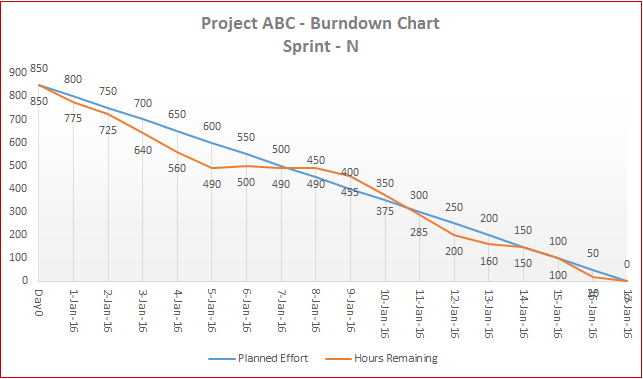
\includegraphics[width=0.5\textwidth]{images/burn_down_chart}
    \caption{Sprint burn down chart}
\end{figure}

\subsubsection{Sprint Retrospective}

The discussion will be on Monday after sprint, and sprint retrospective one of the subject of the meeting. The solution or help will be mention for each individual and the document will be done on Friday.


\subsubsection{Individual Status Reports}

The individual task will be report by each team member every sprint. We will use a share document online to report our process. It will show done or in process.
\subsubsection{Engineering Notebooks}
 
The minimum update of the the engineering notebook will be every meeting on Monday. Each interval will be 5-10 pages as needed, it will depend one how team member working and research about their task. Team will review work submit to keep each member accountable. Every team member except the owner can sign of "witness" for for each ENB page. 
\subsection{Closeout Materials}
The following materials, in addition to major documentation deliverables, will be provided to the customer upon project closeout. Remove this paragraph from your draft, but leave the heading.

\subsubsection{System Prototype}
In the final system prototype, all parts of this project will need to be working. The prototype will consist of the hardware (EE team), firmware (other CS team), and application team (our CS team). It will be due in May, 2020. It will be demonstrated by executing various tests to the Smart Shutters. These tests will be decided on at a later date by the sponsor, Frank Groenteman.


\subsubsection{Project Poster}
The project poster due date has not yet been specified by the instructor. Details will be added at a later date.

\subsubsection{Web Page}
The web page due date has not yet been specified by the instructor. Details will be added at a later date.


\subsubsection{Demo Video}
A demo video will be completed after the prototype is delivered. It will demo all the major functionalities of our application. It will contain video cuts showcasing each functionality. It will only be about 2-3 minutes long.

\subsubsection{Source Code}
Source code will be maintained by everyone in our project using Github. We have yet to discuss how the source code or executable will be presented to the other groups and/or the sponsor.

\subsubsection{Source Code Documentation}
Source documentation will be dependent on the programming language we use. For instance, if you Java is used, we will be generating a Javadoc.






\subsubsection{Installation Scripts}
Installation scripts have not yet been decided. This will be populated once the system requirements, architecture, and design specifications have been completed.

\subsubsection{User Manual}
A digital user manual will be created upon request from the sponsor, Frank Groenteman. Alternatively, the demo video can be provided as the user’s manual.

